%% abtex2-modelo-trabalho-academico.tex, v-1.9.5 laurocesar
%% Copyright 2012-2015 by abnTeX2 group at http://www.abntex.net.br/ 
%%
%% This work may be distributed and/or modified under the
%% conditions of the LaTeX Project Public License, either version 1.3
%% of this license or (at your option) any later version.
%% The latest version of this license is in
%%   http://www.latex-project.org/lppl.txt
%% and version 1.3 or later is part of all distributions of LaTeX
%% version 2005/12/01 or later.
%%
%% This work has the LPPL maintenance status `maintained'.
%% 
%% The Current Maintainer of this work is the abnTeX2 team, led
%% by Lauro César Araujo. Further information are available on 
%% http://www.abntex.net.br/
%%
%% This work consists of the files abntex2-modelo-trabalho-academico.tex,
%% abntex2-modelo-include-comandos and abntex2-modelo-references.bib
%%

% ------------------------------------------------------------------------
% ------------------------------------------------------------------------
% abnTeX2: Modelo de Trabalho Academico (tese de doutorado, dissertacao de
% mestrado e trabalhos monograficos em geral) em conformidade com 
% ABNT NBR 14724:2011: Informacao e documentacao - Trabalhos academicos -
% Apresentacao
% ------------------------------------------------------------------------
% ------------------------------------------------------------------------

\documentclass[
% -- opções da classe memoir --
12pt,				% tamanho da fonte
%openright,			% capítulos começam em pág ímpar (insere página vazia caso preciso)
oneside,			% para impressão em verso e anverso. Oposto a oneside (página em branco = twoside)
a4paper,			% tamanho do papel. 
% -- opções da classe abntex2 --
%chapter=TITLE,		% títulos de capítulos convertidos em letras maiúsculas
%section=TITLE,		% títulos de seções convertidos em letras maiúsculas
%subsection=TITLE,	% títulos de subseções convertidos em letras maiúsculas
%subsubsection=TITLE,% títulos de subsubseções convertidos em letras maiúsculas
% -- opções do pacote babel --
english,			% idioma adicional para hifenização
french,				% idioma adicional para hifenização
spanish,			% idioma adicional para hifenização
brazil				% o último idioma é o principal do documento
]{abntex2}
\usepackage{amssymb}% http://ctan.org/pkg/amssymb
\usepackage{pifont}% http://ctan.org/pkg/pifont
\usepackage{tabularx}
\newcommand{\cmark}{\ding{51}}%
% ---
% Pacotes básicos 
% ---
\usepackage{lmodern}				% Usa a fonte Latin Modern			
\usepackage[T1]{fontenc}			% Selecao de codigos de fonte.
\usepackage[utf8]{inputenc}			% Codificacao do documento (conversão automática dos acentos)
\usepackage{lastpage}				% Usado pela Ficha catalográfica
\usepackage{indentfirst}			% Indenta o primeiro parágrafo de cada seção.
\usepackage{color}					% Controle das cores
\usepackage{graphicx}				% Inclusão de gráficos
\usepackage{microtype} 				% para melhorias de justificação
\usepackage{gensymb}				% Graus Celsius, graus
\usepackage{multicol}				% Multiplas colunas
\usepackage[table,xcdraw]{xcolor}	% Cor na tabela
\usepackage{subcaption}				% Várias figuras
\usepackage{textcomp}				% \textdegree
\usepackage{float}					% Posicionar figuras
\usepackage{url}
\usepackage{grffile}
\usepackage{gensymb}
\usepackage{relsize}
% ---

% ---
% Pacotes adicionais, usados apenas no âmbito do Modelo Canônico do abnteX2
% ---
%\usepackage{lipsum}				% para geração de dummy text
% ---

% ---
% Pacotes de citações
% ---
%\usepackage[brazilian,hyperpageref]{backref}	 % Paginas com as citações na bibl
\usepackage[num]{abntex2cite}	% Citações padrão ABNT
% [num] = citação numérica
% [alf] = citação com nome e ano

% LOCAL DOS ARQUIVOS
%\graphicspath{/home/pedrovdsc/AVES/Relatorio eletrica melhorado}

% --- 
% CONFIGURAÇÕES DE PACOTES
% --- 

% ---
% Configurações do pacote backref
% Usado sem a opção hyperpageref de backref
%\renewcommand{\backrefpagesname}{Citado na(s) página(s):~}
% Texto padrão antes do número das páginas
%\renewcommand{\backref}{}
% Define os textos da citação
%\renewcommand*{\backrefalt}[4]{
%	\ifcase #1 %
%		Nenhuma citação no texto.%
%	\or
%		Citado na página #2.%
%	\else
%		Citado #1 vezes nas páginas #2.%
%	\fi}%
% ---

%----------------------------------------------------------------------------------------
%	TITLE PAGE
%----------------------------------------------------------------------------------------

\newcommand*{\titleGP}{\begingroup % Create the command for including the title page in the document
	\centering % Center all text
	\vspace*{\baselineskip} % White space at the top of the page
	
	\rule{\textwidth}{1.6pt}\vspace*{-\baselineskip}\vspace*{2pt} % Thick horizontal line
	\rule{\textwidth}{0.4pt}\\[\baselineskip] % Thin horizontal line
	
	{\LARGE 	RELATÓRIO \\ [0.3\baselineskip] DIFERENÇAS FINITAS}\\[0.2\baselineskip] % Title
	
	\rule{\textwidth}{0.4pt}\vspace*{-\baselineskip}\vspace{3.2pt} % Thin horizontal line
	\rule{\textwidth}{1.6pt}\\[\baselineskip] % Thick horizontal line
	
	\scshape % Small caps
	%Talvez tentar fazer uma capa mais bonita \\ % Tagline(s) or further description
	%presented  in a clear and useable way \\[\baselineskip] % Tagline(s) or further description
	Vitória,  2019\par % Location and year
	
	\vspace*{7\baselineskip} % Whitespace between location/year and editors
	
	Alunos
	
    {\large João Victor Marçal Bragança\par}
    {\large Pedro Vinicius dos Santos Custodio\par}
   \vspace*{2\baselineskip}
	Professora \\[\baselineskip]
	{\large Andrea Valli \par}
	\vfill
	{\itshape Universidade Federal do Espírito Santo \\ Curso de Engenharia Elétrica\par} % Editor affiliation
	% Whitespace between editor names and publisher logo
	
	% COMENTÁRIO \includegraphics[scale = 0.15]{logo.pdf} \\
	%\plogo \\[0.3\baselineskip] % Publisher logo
	%{\scshape 2012} \\[0.3\baselineskip] % Year published
	% Publisher
	
	\endgroup}


% ---
% Configurações de aparência do PDF final

% alterando o aspecto da cor azul
\definecolor{blue}{RGB}{41,5,195}

% informações do PDF
\makeatletter
\hypersetup{
	%pagebackref=true,
	pdftitle={\@title}, 
	pdfauthor={\@author},
	pdfsubject={\imprimirpreambulo},
	pdfcreator={LaTeX with abnTeX2},
	pdfkeywords={abnt}{latex}{abntex}{abntex2}{trabalho acadêmico}, 
	colorlinks=true,       		% false: boxed links; true: colored links
	linkcolor=blue,          	% color of internal links
	citecolor=blue,        		% color of links to bibliography
	filecolor=magenta,      		% color of file links
	urlcolor=blue,
	bookmarksdepth=4
}
\makeatother
% --- 

% --- 
% Espaçamentos entre linhas e parágrafos 
% --- 

% O tamanho do parágrafo é dado por:
\setlength{\parindent}{1.3cm}

% Controle do espaçamento entre um parágrafo e outro:
\setlength{\parskip}{0.2cm}  % tente também \onelineskip

% ---
% compila o indice
% ---
\makeindex
% ---

% ----
% Início do documento
% ----
\begin{document}
	
	% Seleciona o idioma do documento (conforme pacotes do babel)
	%\selectlanguage{english}
	\selectlanguage{brazil}
	
	% Retira espaço extra obsoleto entre as frases.
	\frenchspacing 
	
	% ----------------------------------------------------------
	% ELEMENTOS PRÉ-TEXTUAIS
	% ----------------------------------------------------------
	% \pretextual
	
	% ---
	% Capa
	% ---
	%\imprimircapa
	\titleGP		% Capa que "fiz"
	% ---
	
	% ---
	% Folha de rosto
	% (o * indica que haverá a ficha bibliográfica)
	% ---
	%\imprimirfolhaderosto*
	% ---
	
	% ---
	% Inserir a ficha bibliografica
	% ---
	
	% ---
	
	% ---
	% RESUMOS
	% ---
	
	% resumo em português
	\setlength{\absparsep}{18pt} % ajusta o espaçamento dos parágrafos do resumo
	%\begin{resumo}
	% O documento aborda a aplicação da mecânica dos fluidos na análise do escoamento sanguíneo. Primeiro, há uma visão geral sobre a fisiologia da circulação. Seguido por propostas de modelos para análise do escoamento. E finalizando com as doenças relacionadas à má condição do sangue e dos vasos sanguíneos.
	
	% \textbf{Palavras-chave}: hemodinâmica. sangue. sanguíneo. %escoamento. fluido. aterosclerose. estenose. bio.
	%\end{resumo}
	
	% resumo em inglês
	%\begin{resumo}[Abstract]
	% \begin{otherlanguage*}{english}
	%   This is the english abstract.
	
	%   \vspace{\onelineskip}
	
	%   \noindent 
	%   \textbf{Keywords}: latex. abntex. text editoration.
	% \end{otherlanguage*}
	%\end{resumo}
	
	
	% ---
	% inserir lista de ilustrações
	% ---
	\pdfbookmark[0]{\listfigurename}{lof}
	%\listoffigures*
	\cleardoublepage
	% ---
	
	% ---
	% inserir lista de tabelas
	% ---
	%\pdfbookmark[0]{\listtablename}{lot}
	%\listoftables*
	%\cleardoublepage
	% ---
	
	% ---
	% inserir lista de abreviaturas e siglas
	% ---
	%\begin{siglas}
	%  \item[ABNT] Associação Brasileira de Normas Técnicas
	%  \item[abnTeX] ABsurdas Normas para TeX
	%\end{siglas}
	% ---
	
	% ---
	% inserir lista de símbolos
	% ---

% ---

% ---
% INSERIR O SUMÁRIO
% ---
\pdfbookmark[0]{\contentsname}{toc}
\tableofcontents*
\cleardoublepage
\settocdepth{section}	% Define o nível do sumário, no caso até 		%						"section"
% ---



% ----------------------------------------------------------
% ELEMENTOS TEXTUAIS
% ----------------------------------------------------------
\textual



\chapter{Introdução}

Neste relatório iremos apresentar a resolução da Equação de Poisson pelo método de diferenças finitas centrais, validando com uma solução já conhecida e resolvendo um problema da área de eletromagnetismo com a solução a ser encontrada pelo método.

\chapter{Validação do Método}

Para validar o método, foi disponibilizado a função:

\begin{center}f(x,y) = $\frac{1}{5}$[x(x-10)+y(y-5)]\end{center}

com as seguintes condições de contorno:
\begin{center}
V = 0 na fronteira. 

V = 0.625x(10-x) para  y = 2.5,  0 $\leq $ x $\leq $  10 
\end{center}

Onde solução conhecida é igual a:

\begin{center}

V(x,y) = $\frac{1}{10}$x(10-x)y(5-y)
\end{center} 

A partir daí, foi implementado um código computacional no Octave a fim de resolver este problema.

Para saber se o código está correto, foi calculado o erro máximo entre a solução conhecida e a solução encontrada. Ela pode ser encontrada a partir da seguinte fórmula.
\begin{center} erro = max|$V_p^{exato}$-$V_p$|, p = 1,2, ... ,$n_x$*$n_y$\end{center}

Utilizando o  método de Gauss-Seidel para encontrar a solução com h = 0.125, foi encontrado que levou 232 iterações para convergir com uma tolerância de $10^{-6}$ com  o tempo de execução de 490.569 seconds.

Utilizando o  método de Gauss-Seidel para encontrar a solução com h = 0.250, foi encontrado que levou 931 iterações para convergir com uma tolerância de $10^{-6}$ com o tempo de execução de 5.4899 seconds.

Utilizando o  método de Gauss-Seidel para encontrar a solução com h = 0.500, foi encontrado que levou 232 iterações para convergir com uma tolerância de $10^{-6}$ com o tempo de execução de 0.0969028 seconds.

Quanto menor o h, maior o tempo de execução pois o gráfico se torna mais fidedigno a realidade e precisa de um maior número de iterações pois a quantidade de pontos a serem calculados aumenta.

Em geral, a escolha do $\omega$ para o método SOR é feita empiricamente, mas em malhas retangulares pode ser encontrada a partir da seguinte fórmula:

\begin{center}$\omega$ =  $\frac{8-\sqrt{64-16t^2}}{t^2}$\end{center}

onde

\begin{center}t = cos($\frac{\pi}{n_x}$)+cos($\frac{\pi}{n_y}$)\end{center}

e $n_x$ e $n_y$ são os números de pontos nas direções x e y.

Para h = 0.125 temos que o $\omega$ ideal é de 1.8856.

Utilizando o  método SOR com $\omega$ = 1.8856 para encontrar a solução com h = 0.125, foi encontrado que levou 162 iterações para convergir com uma tolerância de $10^{-6}$ com  o tempo de execução de 26.0348 seconds.




\newpage




Para h= 0.125, temos os seguintes gráficos:

\begin{figure}[H]
	\begin{center}
		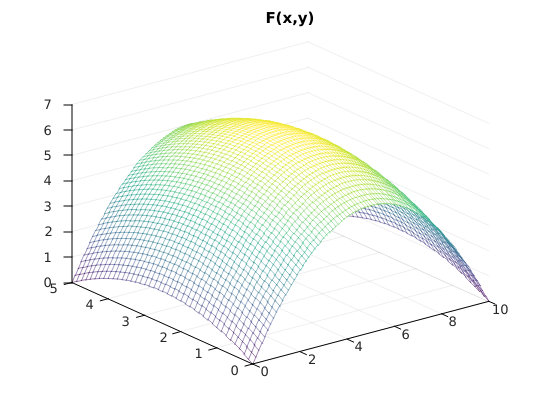
\includegraphics[clip, , width=0.5\linewidth]{validacao_f_h125.png}
		\caption{Função f(x,y) com h = 0.125}
		\label{fluxograma}
	\end{center}
\end{figure}


\begin{figure}[H]
	\begin{center}
		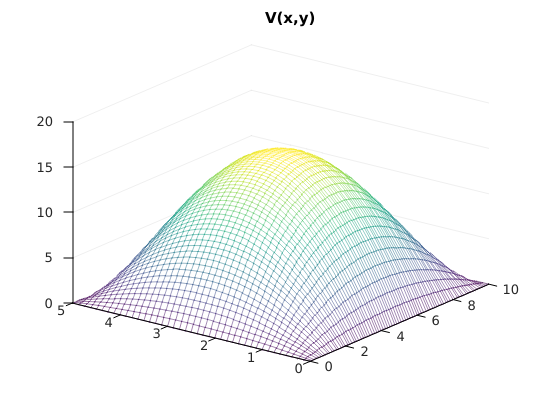
\includegraphics[clip, , width=0.5\linewidth]{validacao_v_h125.png}
		\caption{Função V(x,y) com h = 0.125}
		\label{fluxograma}
	\end{center}
\end{figure}

\begin{figure}[H]
	\begin{center}
		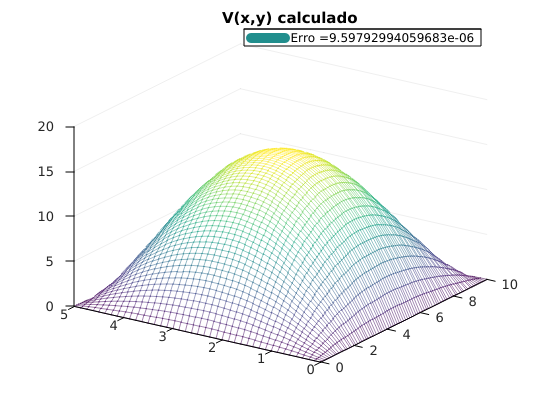
\includegraphics[clip, , width=0.5\linewidth]{validacao_v_calculado_h125.png}
		\caption{Função V(x,y) calculada com h = 0.125}
		\label{fluxograma}
	\end{center}
\end{figure}





\chapter{Capacitor de placas paralelas}

Agora que sabemos que o nosso código está validado, utilizamos em um problema com solução até então desconhecida. O problema está a seguir.

Para um capacitor de placas paralelas, no domínio $\ohm$  = [0,10] $\times$ [0,5], livre de cargas ($\rho$ = 0) e com as condições de contorno:

\begin{center}
V = 0 na fronteira. 

V = +5 para  y = 3,  3 $\leq $ x $\leq $  7

V = -5 para  y = 2,  3 $\leq $ x $\leq $  7
\end{center} 

Foi escolhido para resolver o problema h = 0.125.

\begin{figure}[H]
	\begin{center}
		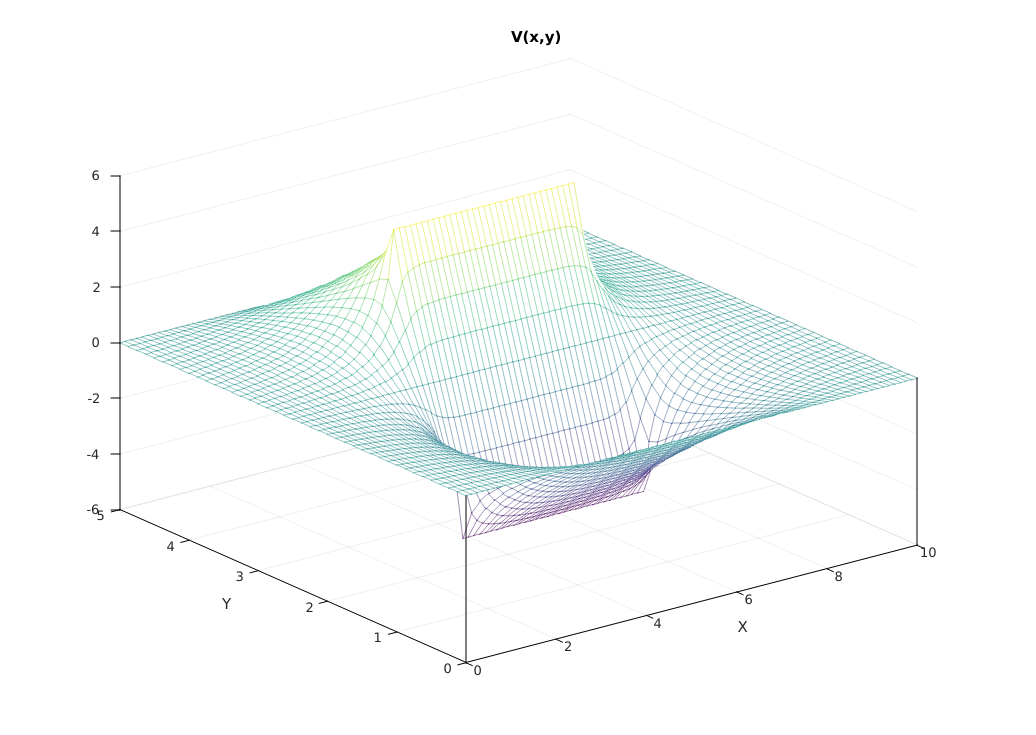
\includegraphics[clip, , width=0.8\linewidth]{capacitor_V_h_125.png}
		\caption{Visão da tensão no capacitor em uma perspectiva 1}
		\label{fluxograma}
	\end{center}
\end{figure}

\begin{figure}[H]
	\begin{center}
		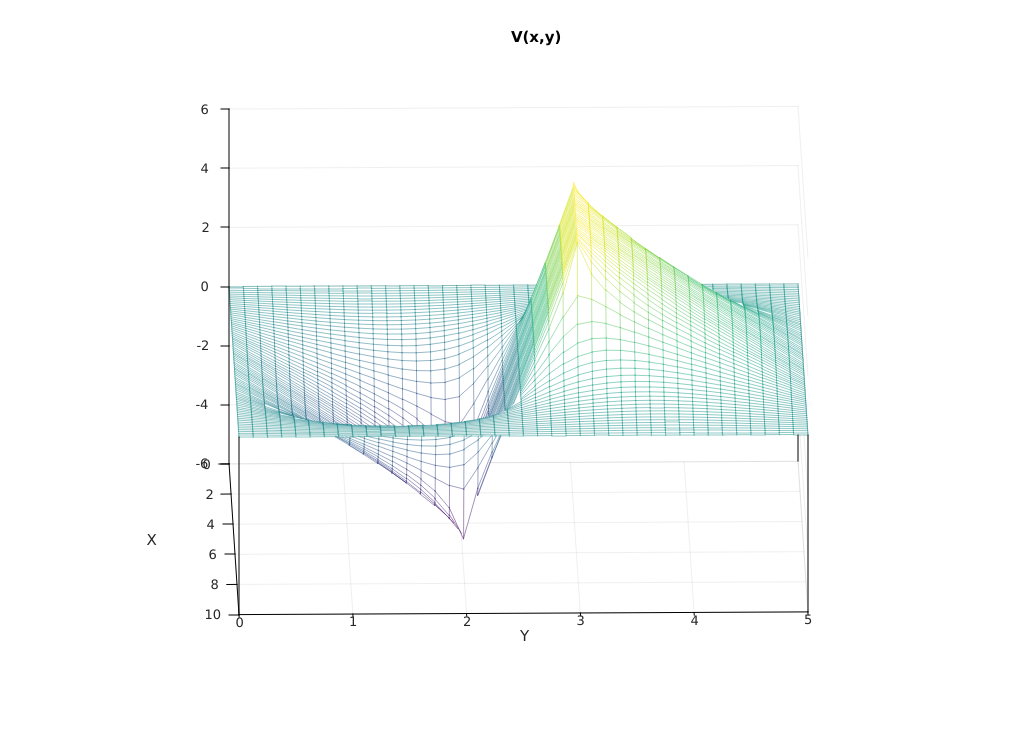
\includegraphics[clip, , width=0.8\linewidth]{capacitor_2_V_h_125.png}
		\caption{Visão da tensão no capacitor em uma perspectiva 2}
		\label{fluxograma}
	\end{center}
\end{figure}

\begin{figure}[H]
	\begin{center}
		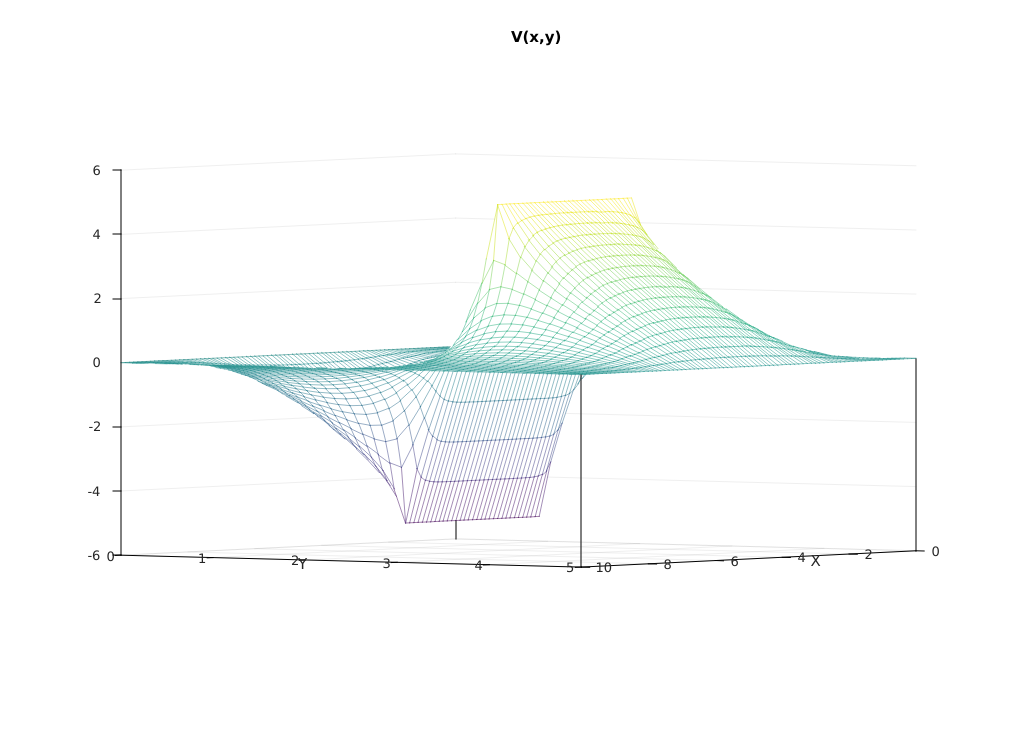
\includegraphics[clip, , width=0.8\linewidth]{capacitor_3_V_h_125.png}
		\caption{Visão da tensão no capacitor em uma perspectiva 3}
		\label{fluxograma}
	\end{center}
\end{figure}

Como se pode observar, as condições de contorno estão atendidas e a tensão no capacitor está variando entre -5V e 5V, o que era de se esperar.

\begin{figure}[H]
	\begin{center}
		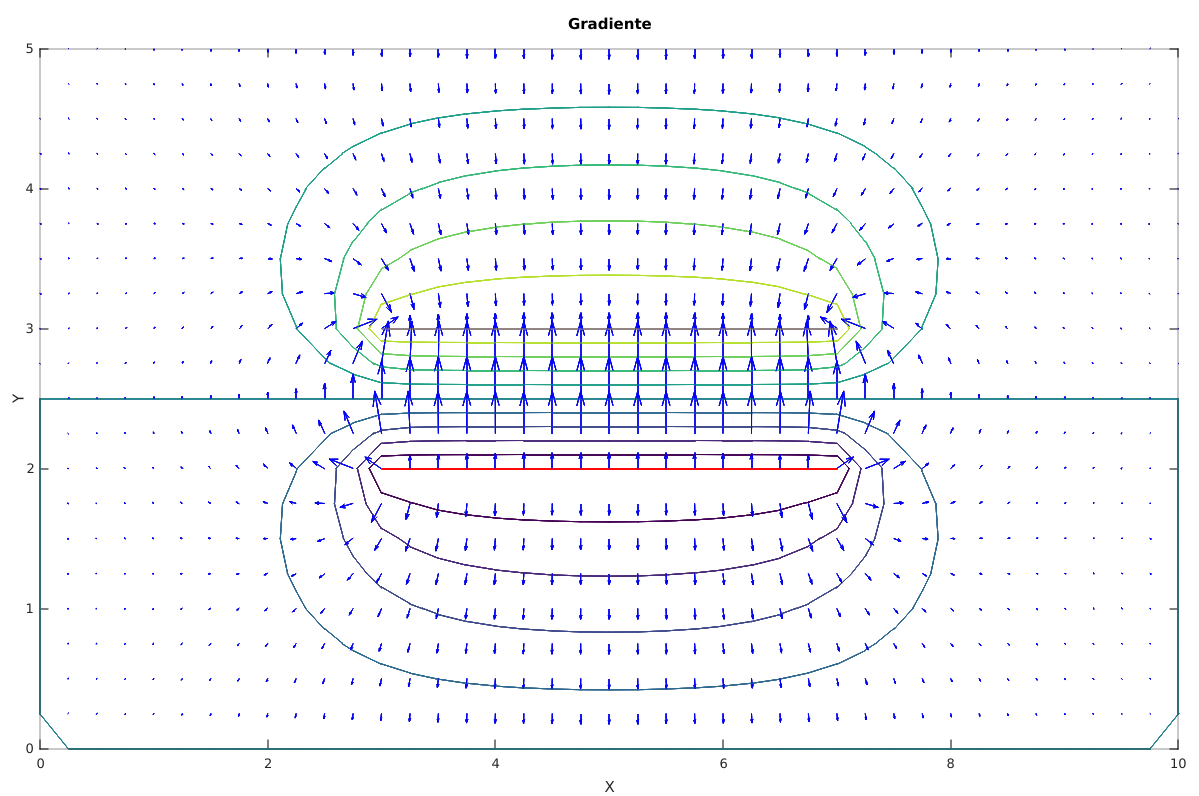
\includegraphics[clip, , width=0.8\linewidth]{contour_capacitor_h125.png}
		\caption{Linhas equipotenciais e gradiente}
		\label{fluxograma}
	\end{center}
\end{figure}

Pela imagem, percebemos que existem regiões elípticas que possuem o mesmo potencial, o que pode-se notar ao fazer cortes horizontais em diferentes alturas no gráfico de tensão do capacitor, e o gradiente mostrando a forma de como a tensão vai aumentando de acordo com a região. As setas sempre vão se aproximando de y = 3 porque o contorno informa que essa região possui tensão de +5V com x variando de 3 a 7 e, as setas sempre vão se afastando de y = 2 porque o contorno informa que essa região possui tensão de -5V com x variando de 3 a 7. Mostrando assim um resultado coerente com o esperado.


\chapter{Resultados}

Os dados obtidos na primeira parte do experimento foram analisados no Matlab usando o \textit{script} fornecido pela professora.

A figura abaixo representa a tensão como uma função $V(x,y)$

\begin{figure}[H]
	\begin{center}
		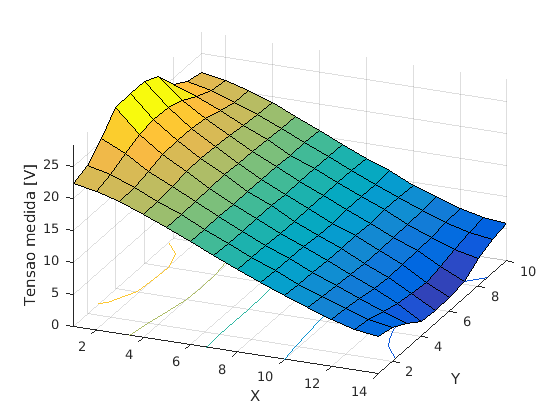
\includegraphics[clip, , width=1\linewidth]{tensao no ponto2.png}
		\caption{Superfície gerada por $V(x,y)$}
		\label{fluxograma}
	\end{center}
\end{figure}

As regiões próximas as placas possuem maior variação de tensão e no centro a variação é bem mais constante, sendo quase linear.

\pagebreak
O \textit{script} também calcula o gradiente da tensão, por consequência, o campo elétrico(\autoref{eq:derivadaComR}), e as linhas equipotenciais.

\begin{figure}[H]
	\begin{center}
		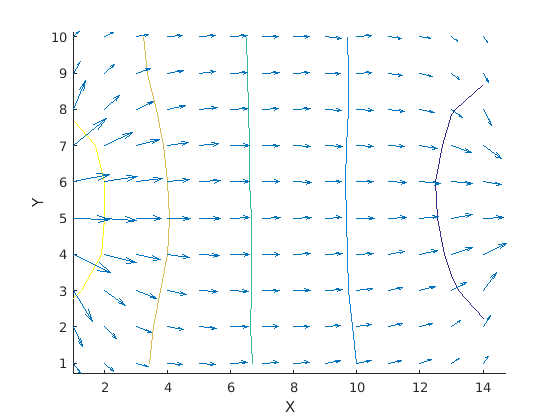
\includegraphics[clip, , width=1\linewidth]{gradiente.png}
		\caption{Gradiente de tensão e linhas de campo elétrico}
		\label{fluxograma}
	\end{center}
\end{figure}

É possível observar que as linhas de campo elétrico são de fato perpendiculares às linhas equipotenciais e que são mais uniformes em sentido e módulo no sentro da cuba.
\pagebreak

Para observar melhor as linhas de campo elétrico e o gradiente de tensão, foi feita uma sobreposição da imagem gerada pelo \textit{script} e de um foto do experimento.

\begin{figure}[H]
	\begin{center}
		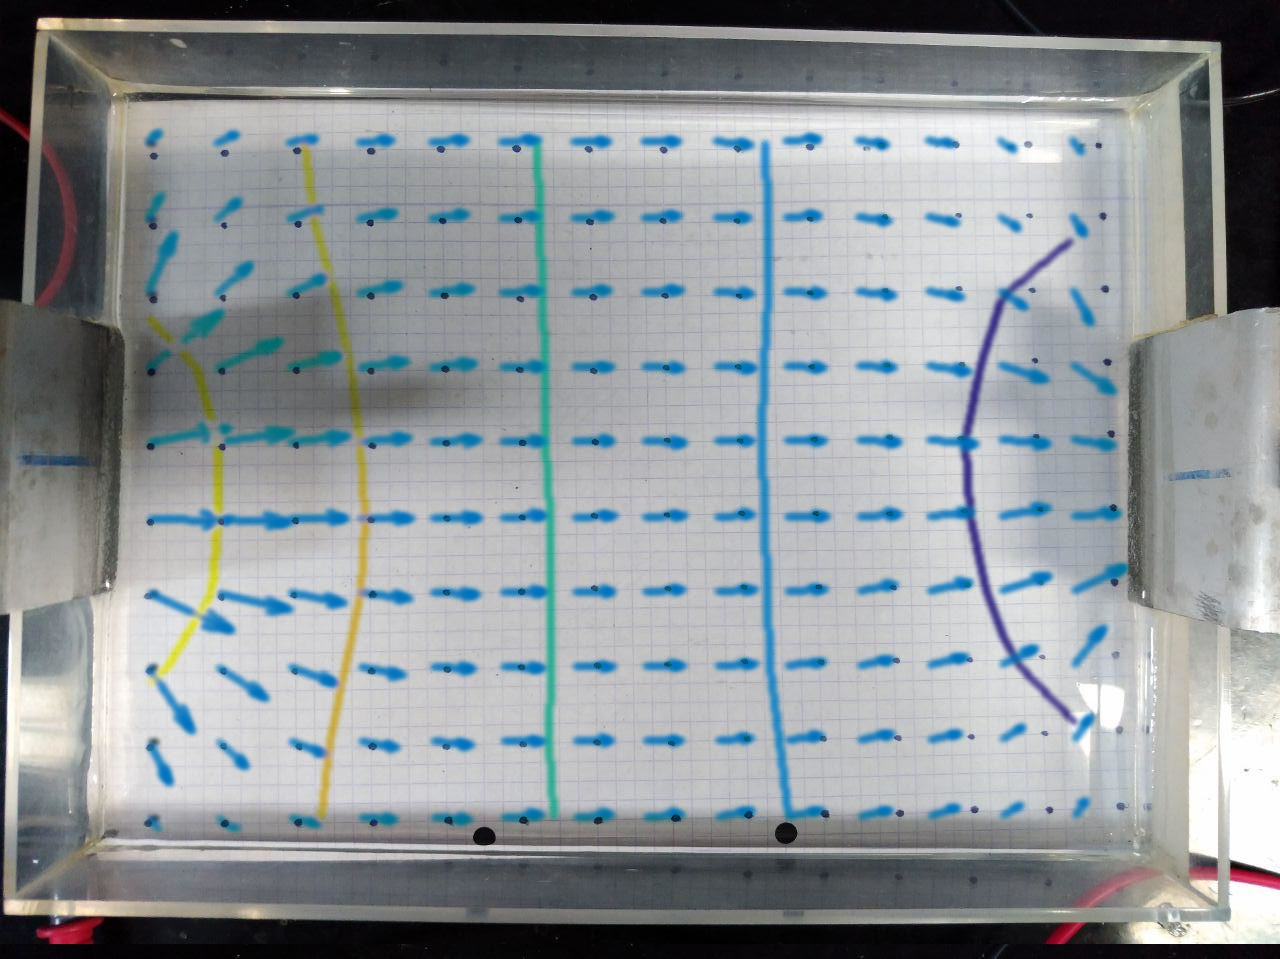
\includegraphics[clip, , width=1\linewidth]{gradiente sobreposto.jpg}
		\caption{Gradiente sobreposto no experimento}
		\label{gradienteSobreposto}
	\end{center}
\end{figure}

Com as imagens sobrepostas, fica mais fácil observar as linhas de campo elétrico divergindo do polo positivo e convergindo para o polo negativo. As linhas equipotenciais também ficam mais evidentes. No centro da cuba elas são mais retas, resultado esperado após a segunda parte do experimento, em que era mais fácil encontrar linhas equipotenciais, pois bastava andar verticalmente com a ponta de prova.

É interessante observar a semelhança do sistema com um dipolo gerado por cargas pontuais, mesmo com a grande dimensão das placas em comparação à distância entre elas.

Apesar de ser possível observar a semelhança anteriormente dita, também é possível observar no centro das placas as linhas de campo normais às superfícies das placas e o efeito de borda nas suas laterais. Como seria esperado numa placa de grande dimensão.

\chapter{Conclusão}

Com o experimento foi possível observar na prática a relação entre o campo elétrico e o potencial elétrico.
Duas coisas saltaram dentre as outras que foram possíveis de serem observadas: as linhas equipotenciais e a semelhança dos resultados obtidos com o de um dipolo gerado por cargas pontuais.
\iffalse
	
\begin{figure}[H]
	\begin{center}
		\includegraphics[clip, , width=1\linewidth]{{fluxograma}.pdf}
		\caption{Fluxograma de aquisição de dados}
		\label{fluxograma}
	\end{center}
\end{figure}
\fi



% ----------------------------------------------------------
% Finaliza a parte no bookmark do PDF
% para que se inicie o bookmark na raiz
% e adiciona espaço de parte no Sumário
% ----------------------------------------------------------
%\phantompart

% ----------------------------------------------------------
% ELEMENTOS PÓS-TEXTUAIS
% ----------------------------------------------------------
\postextual
% ----------------------------------------------------------

% ----------------------------------------------------------
% Referências bibliográficas
% ----------------------------------------------------------

% ----------------------------------------------------------
% Glossário
% ----------------------------------------------------------
%
% Consulte o manual da classe abntex2 para orientações sobre o glossário.
%
%\glossary

\end{document}

